%!TEX root = nonabelions.tex

\chapter{How anyons arise}\label{chap:how anyons arise}

Anyons arise as identical quantum mechanical particles in two dimensions. In order to see how this comes about, we must fist develop the theory of identical particles.








\section{Identical particles and particle statistics}

This discussion is in part based on \cite{myrheim,bonderson}.

Consider $n$ identical quantum mechanical particles. The state of the particles is determined by the wave function
\begin{equation}
  |ψ⟩ : 𝒞ₙ → h
\end{equation}
where $𝒞ₙ$ is the configuration space of the particles, and $h = ℂᵏ$ is the % TODO: the/a ?
local Hilbert space of $k$ local internal degrees of freedom. The configuration space $𝒞ₙ$ is the space of possible spatial positions for the $n$ particles, it is given by
\begin{align}
  𝒞ₙ = \frac{Mⁿ - \bbDeltaₙ}{Sₙ}
\end{align}
where $M$ is the spatial $d$-dimensional manifold on which the particles exist, the set
\begin{align}
  \bbDeltaₙ = \{(x₁,…,xₙ) ∈ Mⁿ ∣ xᵢ = xⱼ \text{ for some } i, j\}
\end{align}
is the set of configurations where particles occupy the same point in space, known as a ``hard-core'' condition.%
\footnote{The hard-core condition is motivated by the fact that without it we cannot say that we have exactly $n$ particles, two of them may be in the same position, thus not visible. Furthermore, if the particles are allowed to be at the same position, they might interact, however, we are not considering particle interactions. In fact, the configuration space is not necessarily a smooth manifold if the singular points of $\bbDelta$ are not removed. In many cases, the points $\bbDelta$ can be added back later in the analysis. The use of hard-core condition has been discussed in depth, see \cite{hard-core} for more details.}
To model the fact that the particles are identical, we form the quotient of $Mⁿ - \bbDeltaₙ$ by the symmetric group $Sₙ$ acting on the coordinates $(x₁,…,xₙ) ∈ Mⁿ$ where $xⱼ$ is the coordinates for the $j$:th particle. In this way all permutations of the $n$ particles are considered to be the same configuration, i.e.\ $(…,xⱼ,…,xₖ,…) = (…,xₖ,…,xⱼ,…)$ in $𝒞ₙ$. Thus, one cannot associate a coordinate $xⱼ$ to a specific particle.









\subsection{Particle exchange: The fundamental group of \texorpdfstring{$𝒞ₙ$}{C\_n}}

Consider exchange of $n$ identical particles with configuration space $𝒞ₙ$. That is, take $n$ identical particles on $M$ with given positions and move them around until they are back at some permutation of the original positions. Since the particles are identical, such an exchange is described by a loop in the configuration space $𝒞ₙ$. More precisely, a loop $γ(t) : [0,1] → 𝒞ₙ$, where $t ∈ [0,1]$ can be seen as the time parameter, corresponds to world-lines of particle trajectories in $M×[0,1]$. The corresponding world-lines are constructed by choosing a representative of $γ(t)$ in $M^n×[0,1]$, e.g.\ associating the coordinates $xⱼ$ with the $j$:th particle, and then projecting the coordinates of each particle into $M×[0,1]$.

In this way, each loop in $𝒞ₙ$ corresponds to a classical motion of the particles along world-lines starting and ending in the same configuration. The corresponding quantum mechanical dynamics is obtained by quantizing the system via the path integral formulation \cite{feynmann path integral,nakahara,feynmann path integrals indistinguishable particles,myrheim}. In this way, homotopically equivalent paths can be seen to give the same contribution. Thus, it is really the fundamental group $π₁(𝒞ₙ)$ of the configuration space that characterize fundamentally different particle exchanges. For more details on this, see \cite{configuration spaces,bonderson}.

What is the resulting state after exchange? Most introductory texts on quantum mechanics give an unsatisfactory discussion of this, not taking the configuration space into account, thus not unraveling anyons.

\begin{example}[Incomplete view of particle exchange]\label{ex:crude exchange}
  The incomplete textbook approach is as follows. Let
  \begin{equation}
    |ψ(…,xⱼ,…,xₖ,…)⟩
  \end{equation}
  be the wave-function of $n$ identical particles. Exchanging particles $j$ and $k$ gives the state
  \begin{equation}
    P_{jk} |ψ(…,xⱼ,…,xₖ,…)⟩ = |ψ(…,xₖ,…,xⱼ,…)⟩.
  \end{equation}
  The probability of measuring a system in the state $|ψ⟩$ is given by $|ψ|²$, since the particles are identical we must then have
  \begin{equation}
    |ψ(…,xₖ,…,xⱼ,…)|² = |ψ(…,xⱼ,…,xₖ,…)|².
  \end{equation}
  Thus
  \begin{equation}
    |ψ(…,xₖ,…,xⱼ,…)⟩ = c |ψ(…,xⱼ,…,xₖ,…)⟩
  \end{equation}
  for some constant $c$. Finally, double exchange returns the state to the original position, i.e. $P_{jk}² = I$, thus
  \begin{equation}
    |ψ(…,xⱼ,…,xₖ,…)⟩ = c² |ψ(…,xⱼ,…,xₖ,…)⟩.
  \end{equation}
  Hence, one concludes $c = ±1$, corresponding to bosons and fermions, respectively.
\end{example}

The flaw in this argument is essentially that double exchange need not return the system to the original state, i.e.\ $P_{jk}² ≠ I$, if the configuration space $𝒞ₙ$ has a non-trivial geometry. To see this clearly, we must specify the notion of particle exchange more precisely.

\begin{definition}[Exchange]
  Consider $n$ identical particles with configuration space $𝒞ₙ$. A path in $𝒞ₙ$ corresponds to motion of the particles, if the path is a loop the particles are returned to a (possibly trivial) permutation of the particles. A non-trivial loop $γ$ corresponds to an exchange of particles, denoted by $P_γ$. Since homotopically equivalent loops are indistinguishable, the exchange operator $P_γ$ is determined only up to homotopy equivalence of $γ$, we may denote the exchange by $P_{[γ]}$ where $[γ]$ is the equivalence class of loops homotopically equivalent to $γ$.
\end{definition}

\begin{definition}[Simple exchange]
  A simple exchange is an exchange where exactly two particles have been exchanged exactly once.
\end{definition}

It is now clear that double exchange $P_γ²$ is trivial if and only if the loop given by traversing $γ$ twice is continuously deformable to the trivial loop, hence returning the state to the original state. As we shall now see, the configuration space need not have this property. This observation is originally due to \cite{leinaas myrheim} in 1976.


% Another way to see that homotopically equivalent paths represent the same physical particle exchange is via the Aharonov-Bohm effect. Particles in two spatial dimensions can be modeled in three dimensions by charged magnetic flux tubes, as these particles move around each other, they gain a quantum phase due to the Aharonov-Bohm effect, this phase is independent of continuous deformations of the path. topological phase <-> magnetic fields.











\subsection{\texorpdfstring{$π_1(𝒞_2)$ with $M = ℝᵈ$}{π₁(C₂) with M = Rᵈ}}\label{sec:conf sp 2 particles}

The configuration space of two identical particles in $ℝᵈ$ is given by
\begin{equation}
  𝒞 = \frac{(ℝᵈ)^2 - \bbDelta}{S_2}.
\end{equation}
The space $(ℝᵈ)^2$ can be factored as $ℝᵈ_\text{cm} × ℝᵈ_\text{rel}$ where $ℝᵈ_\text{cm}$ gives the coordinates of the center of mass for the two particles and $ℝᵈ_\text{rel}$ gives the relative coordinate of the two particles. Let $x_1, x_2 \in ℝᵈ$ be the (absolute) coordinates of the two particles, so that $x = (x_1, x_2) \in 𝒞$. We then define
\begin{equation}
  x_\text{cm} = \frac{1}{2}(x_1 + x_2), \quad
  x_\text{rel} = \frac{1}{2}(x_1 - x_2).
\end{equation}
Now, $Δ = \{(x₁, x₂) ∈ (ℝᵈ)² ∣ x₁ = x₂\}$ is precisely the origin of $ℝᵈ_\text{rel}$.
Furthermore, quotiening with $S_2$ corresponds to quotiening with the antipodal equivalence relation
\begin{equation}
  x ∼ y ⟺ x = -y \text{ or } x = y
\end{equation}
Thus we have
\begin{equation}
  𝒞 = ℝᵈ_\text{cm} × \underbrace{(ℝᵈ_\text{rel} - \{0\}) / {∼}}_{𝒞_\text{rel}}
\end{equation}
and we see that the center of mass contributes trivially to the topology of the configuration space.

The topology of the relative configuration space $𝒞_\text{rel}$ can be understood with the following observation.
The real projective $d$-space is the $d$-sphere with antipodal points identified,
\begin{equation}
  ℝℙᵈ = Sᵈ/{∼}.
\end{equation}
Furthermore, we have $ℝᵈ-\{0\} ≅ ℝ₊ × S^{d-1}$ Thus,
\begin{equation}
  \begin{aligned}
    𝒞_\text{rel}
    &= (ℝᵈ - \{0\})/{∼} \\
    &≅ (ℝ_+ × S^{d-1})/{∼} \\
    &≅ ℝ_+ × S^{d-1}/{∼} \\
    &≅ ℝ_+ × ℝℙ^{d-1}.
  \end{aligned}
\end{equation}

Since the fundamental group has the property that $π_1(X× Y) ≅ π_1(X) × π_1(Y)$ for path connected spaces $X$ and $Y$ we have
\begin{equation}
  π_1(𝒞) = π_1(ℝℙ^{d-1}) =
  \begin{cases}
    ℤ, & d = 2 \\
    ℤ₂, & d ≥ 3
  \end{cases}
\end{equation}
as basic result from topology, showing how the case of two spatial dimensions is special. The fundamental group $ℤ$ can be seen as a way of counting the number of loops, the winding number.

In $d = 2$ dimension the space $𝒞_\text{rel}$ can be seen as the half plane $ℝ^2_{y \ge 0} - \{ 0 \}$ with $x$ and $-x$ identified, geometrically viewed as gluing the edges $ℝ_{-}$ and $ℝ_{+}$ of $ℝ^2_{y \ge 0} - \{ 0 \}$ together. The resulting space can be seen as a punctured cone. In fact, the curvature of this cone can be interpreted to determine the particle statistics.












\subsection{\texorpdfstring{$π_1(𝒞ₙ)$ with $M = ℝᵈ$}{π₁(Cₙ) with M = Rᵈ}}

The above example can be generalized to $n$ particles in $d$-dimensional euclidean space. The corresponding configuration space is then
\begin{equation}
  𝒞ₙ = \frac{\left(ℝᵈ\right)^n - \bbDeltaₙ}{Sₙ}
\end{equation}
and the fundamental group of this configuration space is given by
\begin{equation}
  π₁(𝒞ₙ) =
  \begin{cases}
    Bₙ, & \text{for $d = 2$} \\
    Sₙ, & \text{for $d ≥ 3$}
  \end{cases}
\end{equation}
where $Bₙ$ is the braid group on $n$ strands \cite{fröhlich,khare}.

It is the occurrence of the braid group as the fundamental group for the configuration space for particles in $ℝ²$ that essentially motivate the study of anyons. In \cref{sec:braid group} we define and further discuss the braid group. We disregard other exotic possibilities for the underlying space $M$. For instance, the solid torus is a three-dimensional manifold with fundamental group $ℤ ≅ B₁$. However, this does not really correspond to free particles.

Note that in $d=1$ dimensions, particle exchange of non-interacting particles cannot occur, the configuration space is not connected, it is separated by the removal of $\bbDelta$. In fact, the concept of identical particles is not meaningful in $d = 1$ dimensions, the particles can always be distinguished by which part of the configuration space they exist on, since no transitions can occur, given that particles do not interact. However, one can define generalized statistics by allowing interactions, this gives rise to a rich theory of particle statistics also in one dimension. \cite{polychronakos,myrheim}

















































\section{Representations of \texorpdfstring{$π_1(𝒞ₙ)$}{π₁(Cₙ)} determine particle statistics}

The effect of an exchange of identical particles gives rise to different particle statistics. Since fermions have anti-symmetric wave function, it is clear that two fermions cannot occupy the same state, this is the Pauli exclusion principle, seen as an effective repulsion. On the other hand, bosons have symmetric wave functions and are thus allowed to be in the same state. Statistically it is more likely to find bosons in the same stat than if the particles where distinguishable, seen as an effective attraction. The statistics of bosons and fermions is described by Bose–Einstein statistics and Fermi–Dirac statistics, respectively. Anyons are described by braid statistics, as we shall see in detail.

We have seen that have that particle exchanges, i.e.\ loops in configuration, are distinguished only up to homotopy equivalence. That is, particle exchange must obey the structure of the fundamental group of the configuration space. For instance, if the fundamental group is $Sₙ$, then particle exchange must be such that double exchange is trivial, since $P^2 = 1$ for any element $P$ of $Sₙ$. Thus, it is clear that double exchange in $ℝᵈ$ is trivial for $d ≥ 3$, since the fundamental group of the corresponding configuration space is $Sₙ$. This motivates the crude argument in \cref{ex:crude exchange} for that only fermions and bosons exist, and clarifies when the argument is valid; only for $d \ge 3$ dimensions.

This idea is captured precisely by requiring that particle exchange is determined by a representation of the fundamental group of the configuration space.

\begin{definition}
  A (linear) representation of a group $G$ on a vector space $V$ is a group homomorphism
  \begin{equation}
    ρ : G \mapsto GL(V),
  \end{equation}
  where $GL(V)$ is the general linear group on $V$, i.e.\ the group of automorphisms on $V$.\cite{dummit foote} If $ρ(g)$ commutes with $ρ(h)$ for all $g, h \in G$ we say that the representation is abelian, and say that particles with such exchange are abelian, otherwise we call them non-abelian.
\end{definition}

We shall only be interested in unitary representations, as motivated by the following. The dynamics of every quantum system is determined by the Schrödinger equation
\begin{equation}
  i\frac{∂}{∂t}\ket{ψ(t)} = H\ket{ψ(t)},
\end{equation}
for some Hamiltonian $H$. The solution to this equation is
\begin{equation}
  \ket{ψ(t)} = e^{-iHt}\ket{ψ(0)}.
\end{equation}
Thus, time evolution is given by $U = e^{-iHt}$. Furthermore, time-evolution $U$ of a quantum system must be unitary\footnote{
  Essentially motivated by preserving normalization of quantum probabilities, $|⟨ψ|ψ⟩|² = |⟨Uψ|Uψ⟩|² = |⟨ψ|U^*U|ψ⟩|² ⟺ U^*U = I ⟺ U$ unitary.
}. The operator $U = e^{-iHt}$ is unitary precisely when $H$ is Hermitian.\footnote{Furthermore, the Hamiltonian $H$ must be Hermitian because it is an observable, see \cref{sec:observables}.}

Thus, the result of a particle exchange must be described by a unitary transformation on the Hilbert space $h = ℂᵏ$ of internal degrees of freedom. Therefore, we are only interested in unitary representations on $ℂᵏ$, that is, a map
\begin{equation}
  ρ : G → U(k)
\end{equation}
where $U(k)$ is the group of $k×k$ unitary matrices over $ℂ$.

To sum up:
\begin{lemma}
  The particle exchange operator $P_γ$ must correspond to a unitary representation of $π₁(𝒞ₙ)$, that is
  \begin{equation}
    P_γ |ψ⟩ = ρ(P_γ) |ψ⟩
  \end{equation}
  where $ρ(P_γ)$ is a unitary operator.
\end{lemma}

A representation of the braid group $Bₙ$ need not have the property that $ρ(P_γ)^2 = 1$, a simple example of this is $B₂ ≅ ℤ$ as computed in \cref{sec:conf sp 2 particles}. That is, the wave function need not be invariant under double exchange $P_γ²$. This is due to the non-trivial topology of the configuration space. It is essentially this observation that motivates the study of anyons.

\begin{remark}
  Let $P_γ$ be a simple exchange and assume $π₁(𝒞ₙ) = Sₙ$, we then have that bosons and fermions corresponds to the representations $ρ(P_γ) = 1$ and $ρ(P_γ) = -1$, respectively. In light of this, the question arises: What about other representations of $Sₙ$? As it turns out, the bosonic and fermionic representations are the only one-dimensional representations of $Sₙ$. However, there exists higher-dimensional representations of $Sₙ$. Particles obeying such exchange are sometimes called plektons and their statistics is known as parastatistics. However, it has been shown that parastatistics can always be reduced to bosons or fermions by introducing additional internal degrees of freedom, in the framework of relativistic quantum field theory. \cite{fröhlich,doplicher}
\end{remark}

Thus, if the underlying space is $ℝᵈ$ with $d ≥ 3$, there are fundamentally only two types of particle statistics. However, if the underlying space is $ℝ²$, the fundamental group $π₁(𝒞ₙ)$ is the braid group $Bₙ$ which has much richer representations than $Sₙ$, as we shall see in detail throughout this thesis. Furthermore, statistics arising from higher-dimensional representations of the braid group cannot be reduced to one-dimensional representations, unlike the case of $Sₙ$. \cite{fröhlich}

\begin{remark}\label{rem:fiber bundels}
  The proper way to deal with functions defined on configuration spaces with non-trivial geometry is by using fiber bundles \cite{nakahara}. The state of a quantum system is described by a wave function $ψ$ defined as a section of the vector bundle with fiber $h$ over the configuration space $𝒞$, where $h = ℂᵏ$ is the Hilbert space of $k$ local internal degrees of freedom. In this setting, loops in configuration space that return all particles to the original coordinates need not be homotopically trivial.
\end{remark}





































\section{The braid group}\label{sec:braid group}

The braid group $Bₙ$ is the group with generators $σ₁, …, σ_{n-1}$ and relations
\begin{subequations}
\label{eq:braid relations}
  \begin{align}
    \label{eq:braid relation 1}
    σⱼ σₖ &= σₖ σⱼ, \quad\text{if } |j-k| ≥ 2, \\
    \label{eq:braid relation 2}
    σⱼ σ_{j+1} σⱼ &= σ_{j+1} σⱼ σ_{j+1}.
  \end{align}
\end{subequations}
It is an infinite group, e.g.\ $B₂ = \{σ₁ᵐ: m∈ℤ\}$. The symmetric group $Sₙ$ is defined as the braid group with the additional relation $σⱼ²=1$ for all $j$, it is a finite group.

The braid group can be understood as representing (homotopically equivalent) braids on $n$ strands, the generator $σⱼ$ braids the $j$:th and $j+1$:th strand clockwise, cf.\ \cref{fig:braid group generators}. The braid group relations can thus be visualized as in \cref{fig:braid group rel1,fig:braid group rel2}.

\begin{figure}[!htb]
  \centering
  \begin{tikzpicture}[font=\footnotesize]
    \draw (-1, 0) -- (-1, -1.5);
    \braid[number of strands=4] at s_2^{-1};
    \draw (6, 0) -- (6, -1.5);
    \node at (-1, -1.75) {$1$};
    \node at (0, -0.875) {$\cdots$};
    \node at (1, -1.75) {$j-1$};
    \node at (2, -1.75) {$j$};
    \node at (3, -1.75) {$j+1$};
    \node at (4, -1.75) {$j+2$};
    \node at (5, -0.875) {$\cdots$};
    \node at (6, -1.75) {$n$};
  \end{tikzpicture}
  \caption{Strand representation of the braid group generator $σⱼ$, with time going upwards.}
  \label{fig:braid group generators}
\end{figure}

\begin{figure}[!htb]
  \centering
  \centerline{
  \begin{tikzpicture}[font=\footnotesize,anchor=mid,baseline={([yshift=-.5ex]current bounding box.center)}]
    \braid[number of strands=6] s_4^{-1}s_2^{-1};
    \node at (1, -2.75) {$j-1$};
    \node at (2, -2.75) {$j$};
    \node at (3, -2.75) {$j+1$};
    \node at (4, -2.75) {$j+2$};
    \node at (5, -2.75) {$j+3$};
    \node at (6, -2.75) {$j+4$};
  \end{tikzpicture}
  {\;}={\;}
  \begin{tikzpicture}[font=\footnotesize,anchor=mid,baseline={([yshift=-.5ex]current bounding box.center)}]
    \braid[number of strands=6] s_2^{-1}s_4^{-1};
    \node at (1, -2.75) {$j-1$};
    \node at (2, -2.75) {$j$};
    \node at (3, -2.75) {$j+1$};
    \node at (4, -2.75) {$j+2$};
    \node at (5, -2.75) {$j+3$};
    \node at (6, -2.75) {$j+4$};
  \end{tikzpicture}}
  \caption{Strand representation of $σⱼ σ_{j+2} = σ_{j+2} σⱼ$, illustrating the braid group relation $σᵢ σⱼ = σⱼ σᵢ$ for $|i-j| \ge 2$ in the case $|i-j| = 2$.}
  \label{fig:braid group rel1}
\end{figure}

\begin{figure}[!htb]
  \centering
  \begin{tikzpicture}[font=\footnotesize,anchor=mid,baseline={([yshift=-.5ex]current bounding box.center)}]
    \braid s_1^{-1} s_2^{-1} s_1^{-1};
    \node at (1, -3.75) {$j$};
    \node at (2, -3.75) {$j+1$};
    \node at (3, -3.75) {$j+2$};
  \end{tikzpicture}
  {\quad}={\quad}
  \begin{tikzpicture}[font=\footnotesize,anchor=mid,baseline={([yshift=-.5ex]current bounding box.center)}]
    \braid s_2^{-1} s_1^{-1} s_2^{-1};
    \node at (1, -3.75) {$j$};
    \node at (2, -3.75) {$j+1$};
    \node at (3, -3.75) {$j+2$};
  \end{tikzpicture}
  \caption{Strand representation of the braid group relation $σⱼ σ_{j+1} σⱼ = σ_{j+1} σⱼ σ_{j+1}.$}
  \label{fig:braid group rel2}
\end{figure}

We now define the braid representing exchange of two strands around $p$ fixed strands, which will play a key role when studying statistical repulsion of anyons in \cref{chap:statistical repulsion} and \cref{chap:anyonic braid repr}.

\begin{definition}
  The exchange braid $Σₚ$ is the braid
  \begin{equation}
    Σₚ = σ₁σ₂⋯σₚσ_{p+1}σₚ⋯σ₂σ₁,
  \end{equation}
  on $p+2$ strands, cf. \cref{fig:Up on strands}. This braid keeps the middle $p$ strands fixed while the outer strands $1$ and $p+2$ are exchanged around the middle strands. The corresponding representations is referred to as the exchange operator $Uₚ = ρ(Σₚ)$.
\end{definition}

\begin{figure}[!htb]
  \centering
  \begin{tikzpicture}[font=\footnotesize,anchor=mid,baseline={([yshift=-.5ex]current bounding box.center)}]
    \braid s_1^{-1} s_2^{-1} s_3^{-1} s_2^{-1} s_1^{-1};
    \node at (1, -5.75) {$1$};
    \node at (2, -5.75) {$2$};
    \node at (3, -5.75) {$3$};
    \node at (4, -5.75) {$4$};
  \end{tikzpicture}
  \caption{Strand representation of the exchange operator $U₂ = σ₁σ₂σ₃σ₂σ₁$, note how the middle strands, 2 and 3, are kept in place, while the outer strands 1 and 4 are exchanged.}
  \label{fig:Up on strands}
\end{figure}

The following observation shall later be useful.

\begin{lemma}\label{res:braid generator conjugate}
  All generators of the braid group are conjugate.
\end{lemma}
\begin{proof}
  First, $σᵢ$ is conjugate to $σ_{i+1}$ for all $i$, as seen by
  \begin{equation}
    \begin{aligned}
      (σᵢ σ_{i+1}) σᵢ (σᵢ σ_{i+1})^{-1}
      &= (σᵢ σ_{i+1} σᵢ) σ_{i+1}^{-1} σᵢ^{-1} \\
      [\text{\cref{eq:braid relation 2}}] &= (σ_{i+1} σᵢ σ_{i+1}) σ_{i+1}^{-1} σᵢ^{-1} \\
      &= σ_{i+1} σᵢ σᵢ^{-1} \\
      &= σ_{i+1}.
    \end{aligned}
  \end{equation}
  Finally, conjugation is transitive, thus all braid generators are conjugate.
\end{proof}

As we've seen, the representation of the fundamental group of the configuration space determines the statistics. In $d=2$ dimensions the fundamental group is the braid group. The fact that $Bₙ$ is an infinite group makes the representation theory for $Bₙ$ much more involved than for finite groups. A general discussion of the representation theory of braid groups, see \cite{oskar}. Furthermore, it is not always clear whether a given representation corresponds to physically realizable particles. In this thesis we shall therefore use a general framework of abstract anyon models rooted in quantum field theory to characterize possible non-abelian representations and study the exchange of such anyons, which we introduce in \cref{anyon models}.

A representation $ρ:Bₙ→ℂᵏ$ of $Bₙ$ is determined by $ρ(σⱼ)$ for $j = 1,…,n-1$. If all generator representations commute we say that the representation is abelian. If $k = 1$ the representation is trivially abelian, since $U(1) = \{e^{iθ}:θ∈[0,2π)\}$ is an abelian group. In this case the possible representations are completely characterized by just one parameter $θ$.

\begin{lemma}
  A representation $ρ:Bₙ→ℂ$ is given by
  \begin{equation}
    ρ(σⱼ) = e^{iθ},
  \end{equation}
  for all $j$, with $θ∈[0,2π)$.
\end{lemma}
\begin{proof}
  Since $U(1)$ is an abelian group the second braid group relation \cref{eq:braid relation 2} gives $ρ(σⱼ) = ρ(σ_{j+1})$ for all $j$. The first braid group relation \cref{eq:braid relation 1} is trivially satisfied.
\end{proof}

\begin{remark}
  Since the symmetric group $Sₙ$ is the braid group $Bₙ$ with the additional relation $σⱼ^2 = 1$ we see that one-dimensional representations of $Sₙ$ are such that $ρ(σⱼ) = 1$ for all $j$ or $ρ(σⱼ) = -1$ for all $j$, corresponding to bosons and fermions, respectively.
\end{remark}


All representations $ρ:B₁→ℂᵏ$ of $B₁$ are trivially abelian regardless of the dimension $k$, since there is just one generator $σ₁$. Higher-dimensional representations of $Bₙ$ are generally non-abelian, but not necessarily.

\begin{example}[Higher-dimensional abelian representations] TODO REDO
  Consider $n$ anyons, assume their statistics is determined by an abelian representation $ρ:Bₙ→Cᵏ$ with $k \ge 2$. Since all $ρ(σⱼ)$ commute they can be simultaneously diagonalized. That is, the representation is reducible and can be written as a direct sum of one-dimensional abelian representations, each acting on a separate one-dimensional sector of the Hilbert space $ℂᵏ$. No mixing occurs between these sectors. This situation essentially corresponds to having $k$ different non-interacting one-dimensional abelian anyons, each belonging to one of the sectors.
\end{example}

In this example we saw how non-interacting sectors of the Hilbert space correspond to distinct particle types. This concept gives rise different particle types also in the non-abelian case. The following section discusses this in detail.



































\section{Superselection and particle types}\label{sec:observables}

Before discussing selection and superselection, we must introduce the concept of observables. The set of available observables essentially representing the information that is available for a quantum system.

\subsection{Observables}\label{sec:global vs relative phase}

Everything that can be measured in quantum mechanics is represented by self-adjoint (Hermitian) operators, called observables, acting on the Hilbert space in which the quantum states are defined. A measurement of an observable $A$ on a state $|ψ⟩$ gives exactly one of the eigenvalues $λₐ$ of $A$ (the eigenvalues may have multiplicity) and the resulting state $A|ψ⟩$ after measurement is the projection of $|ψ⟩$ onto the eigenspace corresponding to the measured eigenvalue $λₐ$. Since $A$ is Hermitian, the set of eigenvectors $\{|a⟩\}ₐ$ can be chosen as an orthonormal basis for the space Hilbert space that $A$ acts on. Thus we have a resolution of the identity
\begin{equation}
  I = ∑ₐ |a⟩⟨a|,
\end{equation}
where we assume the Hilbert space to be finite, for the sake of simplifying the discussion. Thus we can write $A$ in its eigenbasis
\begin{equation}
  A = ∑ₐ λₐ |a⟩⟨a|,
\end{equation}
this is essentially the spectral theorem, see for example \cite{reed-simon} for the general version. If $|ψ⟩$ is the quantum state being measured, then we have
\begin{equation}
  ⟨ψ|A|ψ⟩
  = ∑ₐ ⟨ψ|λₐ|a⟩⟨a|ψ⟩
  = ∑ₐ λₐ ⟨ψ|a⟩⟨a|ψ⟩
  = ∑ₐ λₐ |⟨ψ|a⟩|².
\end{equation}
That is, $⟨ψ|A|ψ⟩$ is the expectation value of the measurement of the observable $A$ for the state $|ψ⟩$. In particular, the probability of measuring $λₐ$ is $|⟨ψ|a⟩|²$.

The two quantum states $|ψ⟩$ and $e^{iφ}|ψ⟩$ represent the same physical state. The phase $φ$ of the second state is not physical, it cannot be measured since
\begin{equation}
  ⟨e^{iφ}ψ| A |e^{iφ}ψ⟩
  = e^{-iφ}e^{iφ} ⟨ψ|A|ψ⟩
  = ⟨ψ|A|ψ⟩.
\end{equation}
Such a phase is called a global phase.

A relative phase is a phase ``between'' two states, which can be measured, provided that appropriate observables are available. To illustrate this, consider an orthonormal basis $\{|0⟩, |1⟩\}$ and the general state
\begin{equation}
  |ψ⟩ = ae^{iα} |0⟩ + be^{iβ} |1⟩.
\end{equation}
For a general (Hermitian) observable $A$, the expectation value of a measurement is
\begin{equation}
  \begin{aligned}
    ⟨ψ|A|ψ⟩
    &= a² ⟨0|A|0⟩ + b² ⟨1|A|1⟩ + abe^{i(β-α)}⟨0|A|1⟩ + abe^{i(α-β)}⟨1|A|0⟩ \\
    &= a² ⟨0|A|0⟩ + b² ⟨1|A|1⟩ + abe^{i(β-α)}⟨0|A|1⟩ + ab\overline{e^{i(β-α)}⟨0|A|1⟩} \\
    &= a² ⟨0|A|0⟩ + b² ⟨1|A|1⟩ + 2ab\operatorname{Re}\left(e^{i(β-α)}⟨0|A|1⟩\right) \\
    &= a² ⟨0|A|0⟩ + b² ⟨1|A|1⟩ + 2ab\operatorname{Re}\left⟨0|A|1⟩\right)\cos(β-α)
  \end{aligned}
\end{equation}
The relative phase is $β-α$ and the above shows that it affects measurements for observables with off-diagonal elements, this can be understood as interference. Note that the exact phases $α$ and $β$ can be seen as global phases of $|0⟩$ and $|1⟩$, respectively, explaining why neither can be directly measured.


\subsection{Selection}

Let $|ψ⟩$ is a state of identical particles, then $P_γ|ψ⟩$ cannot be distinguished from $|ψ⟩$ for any exchange $P_γ$. Thus, for any observable $A$ we must have
\begin{equation}
  ⟨ψ|A|ψ⟩ = ⟨ψ|P_γ^*AP_γ|ψ⟩ \quad\text{for all $P_γ$,}
\end{equation}
otherwise the observable $A$ could in principle be used to distinguish the particles. Thus we have the following result.

\begin{lemma}
  If the fundamental group of the configuration space of identical particles is $Sₙ$, all observable of this system must be exchange invariant,
  \begin{equation}
    A = P_γ^*AP_γ\quad\text{for all $P_γ$}.
  \end{equation}
\end{lemma}

This is known as selection rules, for observables of a system of identical particles, effectively giving constraints on what transitions are possible.

Consider particles obeying statistics given by a unitary representation $ρ : π₁(𝒞ₙ) → h$ such that $P_γ ↦ U_γ$. Consider $A$ to be an observable on the local Hilbert space $h$, then we must furthermore have
\begin{equation}
  ⟨ψ|A|ψ⟩ = ⟨ψ|U_γ^*AU_γ|ψ⟩ \quad\text{for all exchange loops $γ$,}
\end{equation}
otherwise the particles would in principle be distinguishable.


\subsection{Superselection}

The obtained selection rules essentially state that the Hilbert space $ℋ$ of a quantum system can be decomposed as $ℋ = ⨂ⱼ ℋⱼ$ where each component $ℋⱼ$ is an invariant subspace for all exchange operators $P_γ$. Since any observable $A$ and $P_γ$ commute, also $A$ leaves these subspaces invariants.
% Furthermore, $A$ and $U_γ$ and thus also for all observables $A$, since $P_γ$ and $A$ commute.
% Furthermore, since $U_γ$ and $A$ commute, also $U_γ$ has $ℋⱼ$ as invariant subspaces.

Thus, with $|ψⱼ⟩ ∈ ℋⱼ$ and $|ψₖ⟩ ∈ ℋₖ$ and $j≠k$, we have
\begin{equation}
  ⟨ψⱼ|A|ψₖ⟩ = 0 = ⟨ψₖ|A|ψⱼ⟩.
\end{equation}
%
% Let $|ψ₁⟩$ and $|ψ₂⟩$ be two states with different exchange symmetry, i.e.
% \begin{equation}
%   \begin{aligned}
%     P_γ |ψ₁⟩ &= U_{1γ} |ψ₁⟩ \\
%     P_γ |ψ₂⟩ &= U_{2γ} |ψ₂⟩
%   \end{aligned}
% \end{equation}
% for $U_γ ≠ U'_γ$. Since any observable $A$ commutes with $P_γ$ we have
% \begin{equation}
%   ⟨ψ|AP_γ|ϕ⟩ = ⟨ψ|P_γA|ϕ⟩ ⟺ ⟨ψ|AU'_γ|ϕ⟩ = ⟨ψ|U_γA|ϕ⟩
% \end{equation}
% but we don't have the equality $AU'_γ = U_γA$ by assumption $U'_γ \ne U_γ$, thus we conclude that
% \begin{equation}
%   ⟨ψ|A|ϕ⟩ = 0
% \end{equation}
% TODO
% for all observables $A$.
%
This is known as superselection, originally introduced by Wick, Wightman and Wigner \cite{wick-wightman-wigner}. The components $ℋⱼ$ of $ℋ$ are known as superselection sectors, or superselection charge sectors, since these sector can be interpreted as different particles types with different `charge'.

An immediate consequence is that there can be no interference between states with different exchange symmetries, since the off-diagonal elements $⟨ψⱼ|A|ψₖ⟩$ of an observable $A$ represent the interference between $|ψⱼ⟩$ and $|ψₖ⟩$. To see this clearly, consider the (not normalized) state
\begin{equation}
  |Ψ⟩ = |ψ₁⟩ + e^{iθ}|ψₖ⟩.
\end{equation}
For any observable $A$ we then have
\begin{equation}
  \begin{aligned}
    ⟨Ψ|A|Ψ⟩
    &= ⟨ψⱼ|A|ψⱼ⟩ + ⟨ψₖ|A|ψₖ⟩ + \underbrace{e^{iθ}⟨ψⱼ|A|ψₖ⟩}_{=0} + e^{-iθ}\underbrace{⟨ψₖ|A|ψⱼ⟩}_{=0} \\
    &= ⟨ψⱼ|A|ψⱼ⟩ + ⟨ψₖ|A|ψₖ⟩
  \end{aligned}
\end{equation}
independent of $e^{iθ}$.

A crude yet vivid example of this is a superposition of a state of two electrons and a state of one electron.

To sum up, states that are superpositions of states from different superselection sectors exhibit no interference, as opposed to superposition states in general. Furthermore, having indistinguishable particles entails that the space of allowed states is a subspace of the full space of distinguishable particle states. The observables that are allowed are those that leave this subspace invariant, they map states of indistinguishable particles to states of indistinguishable particles. Furthermore, superselection implies that all observables leave superselection sectors invariant. Thus, each superselection sector can be understood as a distinct particle type, which cannot be transformed to another particle type. Further discussion of superselection can be found in \cite{ballentine,preskill,kitaev}.





































\section{Interference of anyonic particle exchange}

We shall now see how, in principle, the anyonic exchange operator $U$ of two anyons can be measured. The principle can be illustrated as the quantum circuit in \cref{fig:exchange interference}. Consider a state $|ψ⟩$ of two identical anyons with clockwise exchange given by $|ψ⟩ ↦ U|ψ⟩$. Note that the loop describing clockwise exchange is unique up to homotopy.

\begin{figure}
  \centering
  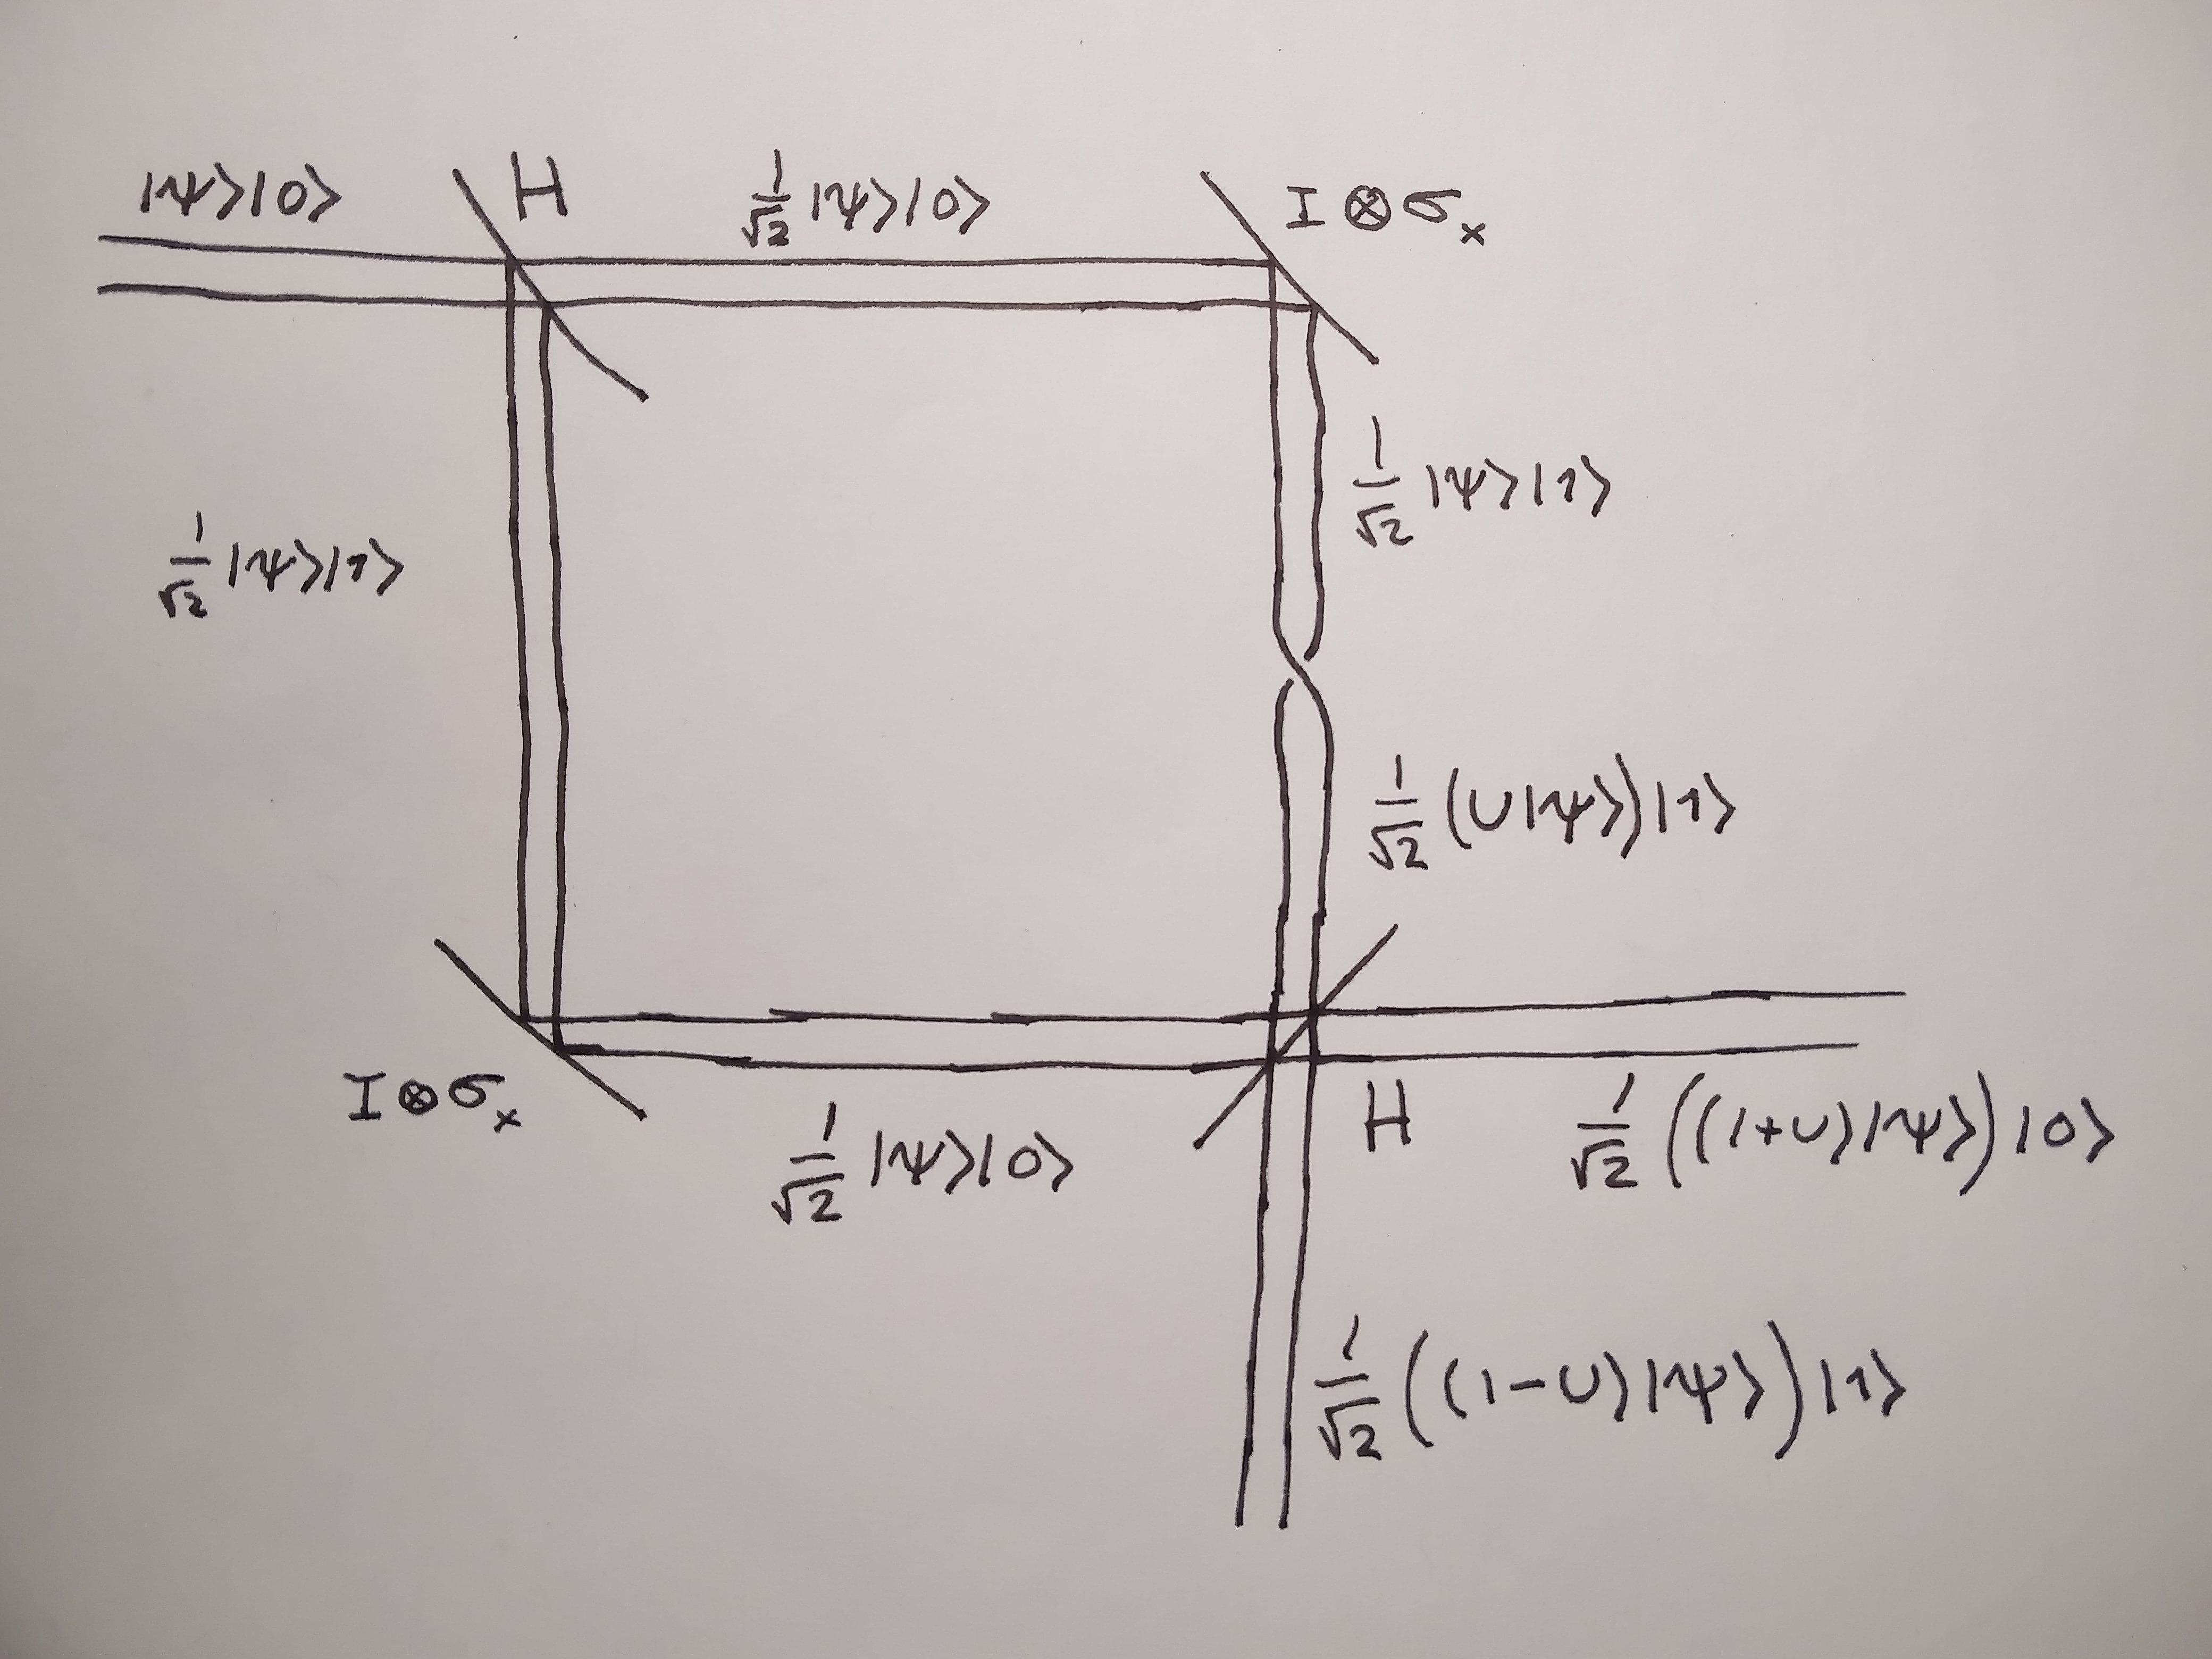
\includegraphics[width=\textwidth]{img/exchange-interference.jpg}
  \caption{Schematic of a quantum circuit to measure the exchange operator $U$ via interference. TODO: Fix $H ↦ I⊗H$ and rotate the final mirror.}
  \label{fig:exchange interference}
\end{figure}

Let $\mathcal{H}_A$ be the Hilbert space of the two anyons and let $|0⟩$ and $|1⟩$ be two orthonormal states, spanning the Hilbert space $\mathcal{H}_B$, in \cref{fig:exchange interference} they represent horizontal and vertical propagation, respectively. Thus, the total Hilbert space is $\mathcal{H} = \mathcal{H}_A⊗\mathcal{H}_B$.

The Hadamard transform defined as
\begin{equation}
  \begin{aligned}
    H : \quad
    \begin{aligned}
      |0⟩ &↦ \tfrac{1}{\sqrt{2}}\big(|0⟩+|1⟩\big) \\
      |1⟩ &↦ \tfrac{1}{\sqrt{2}}\big(|0⟩-|1⟩\big)
    \end{aligned}
  \end{aligned}
\end{equation}
is a unitary transform that forms a superposition of states. Apply the Hadamard transform to the initial state
\begin{equation}
  |ψ⟩⊗|0⟩ \xmapsto{I⊗H} \frac{1}{\sqrt{2}} \Big( |ψ⟩⊗|0⟩ + |ψ⟩⊗|1⟩ \Big).
\end{equation}
Next, apply the unitary operator
\begin{equation}
  \widetilde{U} : \quad
  \begin{alignedat}{4}
    |ψ⟩⊗|0⟩ &{}↦{}& |ψ⟩\phantom{)}&⊗|0⟩ \\
    |ψ⟩⊗|1⟩ &{}↦{}& (U|ψ⟩)&⊗|1⟩
  \end{alignedat}
\end{equation}
that exchanges the particles if they are in the $|1⟩$ state. Note that in \cref{fig:exchange interference} we needed the $I⊗σₓ$ operator where
\begin{equation}
  σₓ : \quad
  \begin{aligned}
    |0⟩ &↦ |1⟩ \\
    |1⟩ &↦ |0⟩
  \end{aligned}
\end{equation}
to recombine the states after the split, this is only for the schematic, mathematically it can be ignored since $σₓ$ simply flips the $|0⟩$ and $|1⟩$ states. The state is thus mapped to
\begin{equation}
  \frac{1}{\sqrt{2}} \Big( |ψ⟩⊗|0⟩ + (U|ψ⟩)⊗|1⟩ \Big).
\end{equation}
Finally, perform a Hadamard transform again, mapping the state to
\begin{equation}
  \frac{1}{2} \Big( \big((I+U)|ψ⟩\big)⊗|0⟩ + \big((I-U)|ψ⟩\big)⊗|1⟩ \Big).
\end{equation}
To sum up we have performed the sequence of three operations $(I⊗H)\widetilde{U}(I⊗H)$. Note that if $U = I$ this sequence of operations does nothing, since $H² = I$.

The exchange phase $U$ can now be measured by performing a measurement in the $\mathcal{H}_B$ space. In the abelian case $U = e^{iθ}$ and the probability of measuring the final state to be in the state $|0⟩$ is
\begin{equation}
  \begin{aligned}
    \abs*{\frac{1+U}{2}}^2
    &= \abs*{\frac{1+e^{iθ}}{2}}^2 \\
    &= \frac{1}{4} \left( 1+e^{iθ} \right) \left( 1+e^{iθ} \right)^* \\
    &= \frac{1}{4} \left( 1 + e^{iθ}e^{-iθ} + e^{iθ} + e^{-iθ} \right) \\
    &= \frac{1}{4} \left( 2 + 2\cos(θ) \right) \\
    &= \frac{1}{2} \left( 1 + \cos(θ) \right).
  \end{aligned}
\end{equation}
The anyonic phase $θ$ can thus be measured, and in this setup $θ$ can be understood as a shift of the probability of measuring the final state in $|0⟩$ or $|1⟩$. In particular, bosons ($θ=0$) always end up in $|0⟩$ and fermions ($θ=π$) always end up in $|1⟩$.

In the case where $U$ is non-abelian, computing the probability of measuring the final state in $|0⟩$ becomes more involved because $U$ can no longer be moved between the two Hilbert spaces $\mathcal{H}_A$ and $\mathcal{H}_B$ as in the case where $U$ is abelian (in which case $U$ is a scalar). We need some more machinery for this, namely that of density operators and partial trace. These concepts are discussed in \cref{sec:density operators and partial trace}. This unfortunate forward reference allows the discussion of quantum computation in \cref{sec:intro qc} to be self-contained.

Denote the resulting state by
\begin{equation}
  |Ψ⟩ = \frac{1}{2} \Big( \big((I+U)|ψ⟩\big)⊗|0⟩ + \big((I-U)|ψ⟩\big)⊗|1⟩ \Big)
\end{equation}
and form the corresponding density operator
\begin{equation}
  ρ_ψ = |ψ⟩⟨ψ|.
\end{equation}
We measure the interference by measuring the probability $P(|0⟩)$ that $ρ_ψ$ is in the state $|0⟩$ in subsystem $B$. The available information of the total state $ρ_ψ$ in subsystem $B$ is given by the reduced density operator $ρ_ψᴮ$ with subsystem $A$ traced out, defined in \cref{eq:red dens op}. Thus,
\begin{equation}
  P(|0⟩) = ⟨0|ρ_ψᴮ|0⟩.
\end{equation}
We have
\begin{equation}
  \begin{aligned}
    ρ_ψ = |Ψ⟩⟨Ψ| =
    \frac{1}{4} \Bigg(
      & \bigg[(I+U)|ψ⟩⟨ψ|(I+U^*)\bigg] ⊗ |0⟩⟨0| {}+{} \\
      & \bigg[(I-U)|ψ⟩⟨ψ|(I-U^*)\bigg] ⊗ |1⟩⟨1| {}+{} \\
      & \bigg[(I+U)|ψ⟩⟨ψ|(I-U^*)\bigg] ⊗ |0⟩⟨1| {}+{} \\
      & \bigg[(I-U)|ψ⟩⟨ψ|(I+U^*)\bigg] ⊗ |1⟩⟨0|
    \Bigg).
  \end{aligned}
\end{equation}
Thus
\begin{equation}
  \begin{aligned}
    ⟨0|ρ_ψᴮ|0⟩_B
    &= \frac{1}{4} \operatorname{tr} \Big[(I+U)|ψ⟩⟨ψ|(I+U^*)\Big] \\
    &= \frac{1}{4} ∑ₖ ⟨k|(I+U)|ψ⟩⟨ψ|(I+U^*)|k⟩ \\
    &= \frac{1}{4} ∑ₖ |⟨k|(I+U)|ψ⟩|².
  \end{aligned}
\end{equation}

We recover the result for abelian anyons by letting $U = e^{iθ}$,
\begin{equation}
  \begin{aligned}
    ⟨0|ρ_ψᴮ|0⟩_B
    &= \frac{1}{4} ∑ₖ |⟨k|(I+U)|ψ⟩|² \\
    &= \frac{1}{4} ∑ₖ |1+e^{iθ}|² |⟨k|ψ⟩|² \\
    &= \frac{1}{2} (1+\cosθ),
  \end{aligned}
\end{equation}
where $∑ₖ |⟨k|ψ⟩|² = 1$ due to normalization of $|ψ⟩$.

For general $U$ it is difficult to say much more than this. The dependence of the probability $⟨0|ρ_ψᴮ|0⟩$ on the exchange operator $U$ can be rather involved. Assuming that we have control of the state $|ψ⟩$, with an appropriate set of choices for $|ψ⟩$ the elements of $U$ can be deduced by repeating the interference measurement. We outline this idea in the following example.

\begin{example}
  Let $ℋ_A$ be two-dimensional. We can then write
  \begin{equation}
    |ψ⟩ = c₀|0⟩ + c₁|1⟩
  \end{equation}
  and
  \begin{equation}
    U =
    \begin{pmatrix}
      u_{00} & u_{01} \\
      u_{10} & u_{11}
    \end{pmatrix}
    =
    \begin{pmatrix}
      a & b \\
      -e^{iθ}b^* & e^{iθ}a^*
    \end{pmatrix}
  \end{equation}
  Thus we have
  \begin{equation}
    \begin{aligned}
      ⟨0|ρ_ψᴮ|0⟩_B
      &= \frac{1}{4} \left( |(u_{00}+1)c₀ + u_{01}c₁|² + |u_{10}c₀ + (u_{11}+1)c₁|² \right) \\
      &= \frac{1}{4} \left( |(a+1)c₀ + bc₁|² + |-e^{iθ}b^*c₀ + (e^{iθ}a^*+1)c₁|² \right).
    \end{aligned}
  \end{equation}
  Determining $U$ amounts to determining four real parameters, $\operatorname{arg}(a)$, $\operatorname{arg}(b)$, $|a|$ and $θ$. For example, the choice $|ψ⟩=|0⟩$ gives
  \begin{equation}
    \begin{aligned}
      ⟨0|ρ_ψᴮ|0⟩_B
      &= \frac{1}{4} \left( |a+1|² + |-e^{iθ}b|² \right) \\
      &= \frac{1}{4} \left( |a|² + 1 + 2\operatorname{Re}(a) + |b|² \right) \\
      &= \frac{1}{2} \left( 1 + \cos(\operatorname{arg}(a)) \right),
    \end{aligned}
  \end{equation}
  allowing measurements of $\operatorname{arg}(a)$.
  Similarly, the other parameters of $U$ can be determined by appropriately choosing the state $|ψ⟩$.

  If we work in the eigenbasis of $U$ we have
  \begin{equation}
    U =
    \begin{pmatrix}
      e^{iθ₁} & 0 \\
      0 & e^{iθ₂}
    \end{pmatrix}
  \end{equation}
  and then
  \begin{equation}
    ⟨0|ρ_ψᴮ|0⟩_B = \frac{1}{2} \left( |c₀|²(1+\cos(θ₁)) + |c₁|²(1+\cos(θ₂)) \right).
  \end{equation}
\end{example}

This procedure can be straight-forward extended to let the the state $|ψ⟩$ represent more than two anyons, and thus allow the operator $\widetilde{U}$ to introduce a more complex braid. In this way, truly non-abelian properties of a larger system of anyons can in principle be probed.

Other methods of anyonic interferometry is discussed in \cite{bonderson}. Note that as one anyon is taken around one or several other anyons, the introduced phase can only be measured after one full loop as been traversed and the phase can be compared to another anyon. Thus, it is not physical to say that the phase continuously (or in any other way) changes during the exchange. That is, how the phase is affected before the particles meet is non-physical, we are free to choose this as long as the choice respects the result of a complete winding of particles; this illustrates the gauge invariance of the anyonic phase during braiding.









































\section{Anyon models and physical realizability}\label{sec:models and realizability}

This thesis focuses primarily on the mathematical aspects of anyons, however, in this section we give a short account of possible physical realizations for anyons. This topic is further discussed in for instance \cite{nayak,topological quantum compiling,slingerland bais}.

Abelian anyons have been claimed to have been detected in the fractional quantum hall (FQH) effect \cite{abelian fqh}. These results are not unambiguous and total consensus does not exist in the scientific community. It is  Furthermore, it has only been conjectured that non-abelian anyons can be realized in FQH liquids at the filling fractions $\nu = 5/2$, where anyons known as the Ising anyons are thought to exist \cite{wang book}. Partial experimental results exist which support the existence of non-abelian anyons \cite{non-abelian experimental}. The Fibonacci anyon model which is studied in \cref{fibonacci anyons} has support from the topological quantum field theory $SU(2)₃$ Chern-Simons-Witten (CSW). \cite{nayak}

There are different attempts to identify whether particles obey anyonic statistics. Interferometry methods have been developed, as in \cite{bonderson}. Another approach is to study the wave function density, as outlined in \cite{lundholm-rougerie,fractional angular momentum}. The benefit of using interferometry is that it is a direct way to identify braid statistics, while the wave function density is an indirect effect of the statistics. However, anyonic interferometry is in practice difficult to achieve, it can be argued that wave function density is easier to measure.

In the literature one generally encounters two types of anyons.
\begin{enumerate}
  \item Anyons with quantum dynamics, giving rise to anyonic particle statistics, i.e. braid statistics. Such particles must necessarily be allowed to move freely in space, such as in a gas. This is the type of anyons that one has in mind when discussion statistical repulsion.
  \item Anyons with fixed or controlled coordinates. In the strict sense this can be any quantum system that is governed by a representation of the braid group. This is the type of anyons that one has in mind when discussing the use of anyons for topological quantum computation. The anyons need to be fixed so that controlled braiding can be performed. In principle this can be achieved by forcing the position of dynamical anyons by placing each anyon in a deep potential that can be externally controlled.
\end{enumerate}
